\documentclass[a4paper]{article}
\usepackage[utf8]{inputenc}
\usepackage[margin=1in]{geometry}

\title{Final report lab Distributed Systems}
\author{Authors \\ Rick Proost  (rpjproost@gmail.com)\\  Dorian de Koning (doriandekoning@gmail.com)  \\ Support cast}
\date{March 2018}

\usepackage{natbib}
\usepackage{graphicx}
\graphicspath{ {images/} } 

\begin{document}

\maketitle

\begin{abstract}
    Simulating distributed systems is a problem with a high computational complexity, therefore the feasibility of distributed simulators for distributed systems is investigated and reported in this paper.
    \cite{adams1995hitchhiker} % TODO: !!!REMOVE THIS CITE!!! (compilen op mn pc via VSC lijkt alleen te werken als ik references.bib uit comment of iig 1 cite doe, deze kan weg als we andere citatie hebben)
    
\end{abstract}

\section{Introduction}
The vast majority of internet services nowadays rely on cloud services, these cloud services often rely on multi-cluster systems which can be placed in different geographical locations. 
To aid development of these complex distributed systems many companies invest in experimental setups for multi-cluster simulation. 
Unfortunately computational complexity of these simulators is high.\\

Several solutions already exist for this problem [TODO description existing systems and tools]\\%http://simgrid.gforge.inria.fr/

In this paper the design and implementation of distributed simulation of a distributed grid scheduler is discussed. 
This system can be used by users to conduct research on distributed systems without the need for costly physical setups. 
A simulator which simulates such a system with only a single grid scheduler is available for study.\\
In the next section some background on the implemented application and its main requirements will be provided, after this the design of the implemented system will be discussed. 
Where after experiments and their results conducted on the implemented system will be discussed. 
The report ends with a discussion summarising the main findings of this work and a conclusion.

\section{Background on Application}
This section will provide some background on the implemented application as well as the main requirements that need to be fulfilled. 
Virtual grid system simulators (VGS) are complex systems that simulate distributed systems. The simulated system consists of many clusters and several grid scheduler nodes. 
These clusters consist of a vast amount of compute nodes and a resource manager which handles the allocation of resources. 
Each resource manager has a fixed amount of compute nodes to distribute jobs to.
Clients can send jobs to be executed to these clusters, when a job arrives at the resource manager, the resource manager will add it to its queue from where it can be dispatched to idle compute nodes. 
Because of imbalanced loads or resource manager failures these clusters are interconnected via grid schedulers which enable load sharing among clusters. 
When one of the clusters has a higher workload then other clusters, jobs can be distributed equally among clusters by load balancing via the grid schedulers. 
These grid schedulers should also provide a degree of protection against resource manager crashes by providing replication.\\

\section{Requirements}
In this section the main requirements of the system build will be further explained.
These requirements will always hold for the virtual gridscheduler system and form the foundation for all the techniques implemented.

\subsection{Operational requirements}
Every gridscheduler maintains its own job queue and every resource manager maintains its own job queue, the resource managers queue is limited to a fixed size, its node capacity plus 25 percent.
All jobs initially arrive at a resource manager, which can be the same one for all jobs, but also chosen randomly.
At most one gridscheduler and at most one resource manager can crash at a time to prevent loss of jobs.
The system functions when more crashes occur, however some jobs given by the client could be lost and never completed.

%consistency requirements
\subsection{Consistency}
The system needs to fulfil several requirements. 
First of all jobs that arrive in a resource manager should be executed within a reasonable amount of time but not executed more than once, i.e. no jobs should get lost or duplicated once they are in the system. 
Therefore no job can be present in multiple grid scheduler or resource manager queues at any point in time. 

%scalability
\subsection{Scalability}
Another requirement is posed on scalability of the system, 
to accommodate for multiple users using the system at the same time or users executing complex simulations the system should be able to run with at least 5 grid scheduler nodes, 20 clusters with at least 1.000 compute nodes. 
To provide the ability to study realistic load imbalance simulations the ratio of the amount of jobs arriving at resource managers should be at least 5. \\
% fault tolerance
\subsection{Fault tolerance}
To realistically simulate a distributed system single grid scheduler and resource manager nodes may crash and restart, the system should continue to function correctly after a node has crashed. 
When a node restarts their job queue should restored using logs stored on other grid schedulers, no jobs may get lost. 
Therefore events that happen within the system, like job arrivals, job starts, job completions and node restarts should be logged on at least two grid scheduler nodes. 

%auxiliary

\section{System design}
In this section more in-depth information is provided on how certain requirements from the previous section are implemented to ensure a valid system.
Consistency, scalability and fault tolerance strategies are explained. 
Also the limitations of the system will be reviewed here.

\subsection{Overview}
Figure [xx] shows an overview of the system, containing in this example, three gridschedulers, three resource managers and a lot of nodes per cluster.
In this design it is important to notice that all gridschedulers are interconnected, and all resource managers to all gridschedulers, but resource managers are not interconnected.
Also gridschedulers will never broadcast to resource managers because of scalability issues, gridschedulers do broadcast to eachother and resource managers can broadcast to gridschedulers.
The reason for allowing broadcasting towards gridschedulers is because the assumption is made that within this ecosystem, it is far more realistic to have a low amount of gridschedulers and a lot of clusters. \\
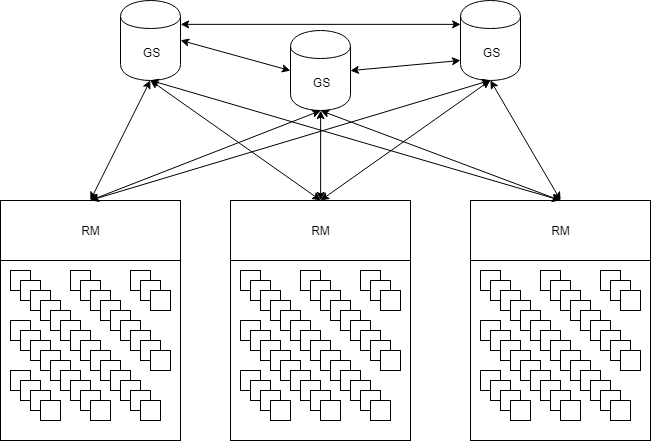
\includegraphics[scale=0.5]{design-overview.png}

Gridschedulers and resource managers have their own job queue, however the queue for the resource manager is limited because if the treshold of incoming jobs is reached, the resource managers will offload to the gridschedulers.
Load-balancing can then ben done by the gridschedulers. 
The gridschedulers keep track of the least loaded resource manager through messages received from the resource managers, every message that is sent from a resource manager will always contain the current load of that resoure manager.
Therefore every gridscheduler has a rough estimate of which resource manager maintains the least loaded cluster, and the gridscheduler will then pick that resource manager to do the job it wants to dispatch. \\

Every resource manager and gridscheduler also gives every message it sents a sequence ID, this can be used to backtrack in which order actions occurred on that respective gridscheduler or resource manager.
For the design of this system there was no need to synchronize these sequence IDs amongst the different gridschedulers or resource managers while it is only important to know how a certain queue can be recreated in the right order.
For that only information of a single entity in the system is needed and then a sequence ID per entity is enough to reconstruct the queue.

\subsection{Resource manager scheduling}
A client will always send a job to a cluster, where a resource manager will pick up the job. 
In the case of the example in figure [xx] a resource managers queue is below the treshold where it will offload the job.
The treshold is defined by the capacity of the computational nodes in the resource managers cluster plus 25 percent.
In the case that a resource manager has capacity for the incoming job, it will put the job in its own queue and broadcast to all gridschedulers it retrieved the job.
Now the gridschedulers take notice and put the job in the log for that resource manager, every gridscheduler has a log for every resource manager in the system. \\
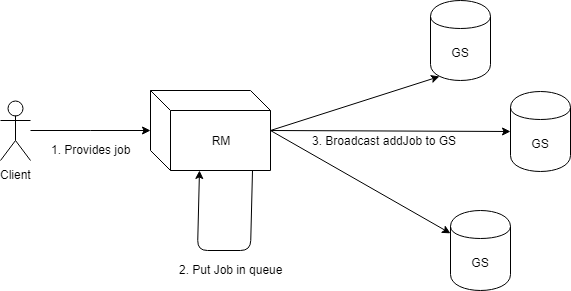
\includegraphics[scale=0.5]{design-rm-own-queue.png}

Another example is given in figure [xx], in this case the resource managers load is above the treshold and in this case it will offload to a random gridscheduler.
When the gridscheduler retrieves the job, it will sent a request to add the job to its queue to another gridscheduler, if that message is acknowledged the action is logged in atleast two gridschedulers.
If an acknowledgement is never sent, it is detected by the gridscheduler sending the request by a thread that will check if the request was sent withing five seconds from now, otherwise pick another gridscheduler and request permission to add the job to its queue.
Now if any acknowledgement is retrieved, atleast one other gridscheduler can help recreate the queue of the requesting gridscheduler. \\

This request can also be broadcasted, then if one gridscheduler fails, all the others could potentially have the power to recreate the queue of the requesting gridscheduler, however scalability issues will arise.
Logs will be saved in all gridscheduler for all gridschedulers which is a lot of data, this could be garbage collected when job finished messages arrive.
Another problem for scalability will be the channels between gridschedulers will get full when a lot of small jobs will be added in a short time, therefore the single cast method is chosen. \\

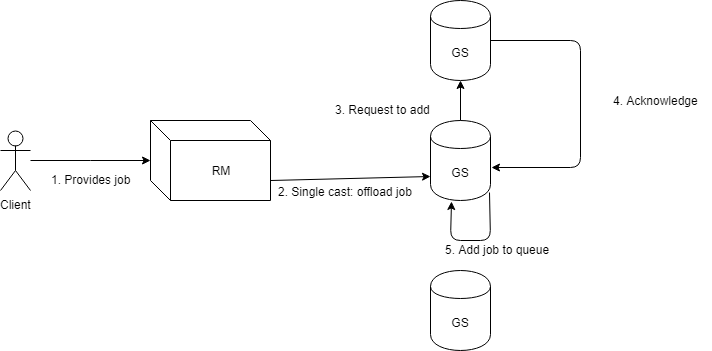
\includegraphics[scale=0.5]{design-rm-offload-job.png}

\subsection{Gridscheduler scheduling}
As described in the general overview of the system, the gridscheduler keeps track of the least loaded resource manager by updating the load in its hashmap of the resource managers with the load retrieved in every message that it gets from 
that resource manager.
As can be seen in figure [xx] a request is made to another gridscheduler to dispatch the job to a certain resource manager, which job and which resource manager is information contained in the message.
If the request does not get a message in time, this is checked in the same way as mentioned in the previous subquestion, the request to dispatch is sent to another gridscheduler. 
When the acknowledgement is received, the job is dispatched to the specified resource manager.
The resource manager will always accept the job and put it in its queue, an acknowledgement is sent from the resource manager to the gridscheduler, also containing its current load which is important for the load-balancing.
\\
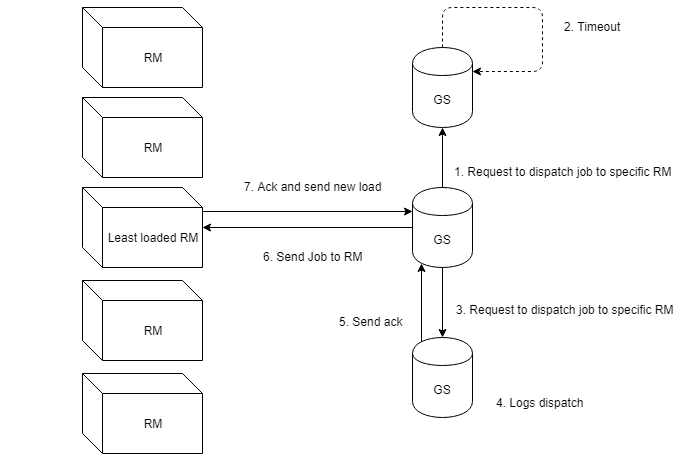
\includegraphics[scale=0.5]{design-gs-dispatch-job.png}


\subsection{Fault tolerance}
This subsection will describe how certain parts of the system can crash without losing functionality in the system.
Within some predefined boundaries, the system will not lose any jobs and/or information about the state and queues of the system.
The predefined boundaries in the system are that at most one gridscheduler and at most one resource manager can crash at a time to fully recover.
However the system will still function when more crashes happen at once, only the chance on loss of jobs given by the client will be there. \\

\subsubsection{Node crashes}
Whenever a node crashes the resource manager will detect the state of the node, in the event logs of the resource manager it will recover the job that was given to that node and it will add it to its own queue.
Therefore the node that has crashed does not have to restart to complete the job, if the node restarts it will just be given jobs from the queue of the resource manager again.
This is the easiest crash to recover from in the system.

\subsubsection{Resource manager crashes}
Figure [xx] shows what happens whenever a resource manager crashes. 
In this system we assume that a resource manager and/or gridscheduler that crashes will always come back online.
It does not matter how long this restart takes, or if another physical unit is started with the same resource manager or gridscheduler ID, but if that ID is started again, the queueu will recover.
Figure [xx] depicts that after restarting the resource manager broadcasts to get its log to all gridschedulers, the log will then be sent from all gridschedulers to that resource manager.
In the moment it is retrieving those logs, it is in an recovering state and will not take jobs from any of the gridschedulers.
When logs are received from all gridschedulers, the queue can be recovered for the resource manager and while the sequence IDs of that resource manager are in the logs, the same order can be achieved in the queue as before. \\
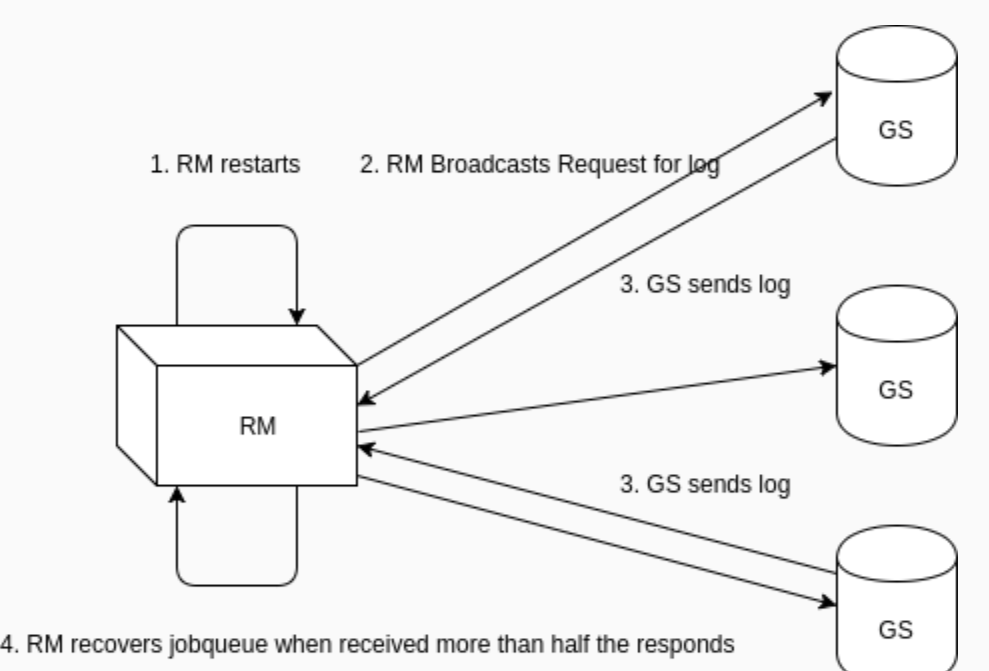
\includegraphics[scale=0.5]{design-rm-crash.PNG}

\subsubsection{Gridscheduler crashes}
The gridscheduler crashes work almost the same as the resource manager crashes, the gridscheduler broadcasts to all other gridschedulers and together with the sequence IDs in the log it will recover its queue in the same order as before.
Note that if another gridscheduler would be down at the same time, there is a chance that not all the jobs can be recovered, however the system will still function and continue.

\subsection{Realistic experiments}
The system virtually recreates a distributed grid, to do realistic experiments a parser is written for GWF files. 
GWF files are Grid Workload Format files and they contain information on which computational unit retrieves a certain job, how long a job takes, when it is given to the cluster by the client, etc.
By parsing GWF files that represent realistic workloads retrieved from http://gwa.ewi.tudelft.nl/datasets/, a certain degree of realism can be simulated on the system.

\subsection{Repeatability}
Another way of feeding jobs by the client to the system is done via a random workload provider, this is a provider written to work in the same way as the GWF files.
Crashes can be fed into the system, aswell as delays and speedups.
For making sure we can run tests on the same input over and over again the random workload provider always outputs a file just like the other GWF files which can then be parsed again and fed to the system.


\section{Experimental Results}
http://gwa.ewi.tudelft.nl/datasets/gwa-t-1-das2/report/

\section{Discussion}

\section{Conclusion}


\bibliographystyle{plain}
\bibliography{references}
\end{document}
